\documentclass[11pt, twocolumn]{article}
\usepackage[letterpaper, margin=0.5in]{geometry}
\usepackage[utf8]{inputenc}
%\usepackage[document]{ragged2e}
\usepackage[parfill]{parskip}
\usepackage[font=small, margin=1cm]{caption}

\usepackage{epsfig} %% for loading postscript figures
\usepackage{amsmath}
\usepackage{amssymb}
\usepackage{fancyhdr}
\usepackage{changepage}
\usepackage{enumerate}
\usepackage{graphicx}
\usepackage{titling}
\usepackage{float}
\usepackage{csquotes}

\usepackage{titlesec}
\usepackage{titling}

\titleformat*{\section}{\LARGE\sffamily}
\titleformat*{\subsection}{\Large\sffamily}
\titleformat*{\subsubsection}{\large\sffamily}
\renewcommand{\maketitlehooka}{\sffamily}

\graphicspath{{figures/}}

\title{%
  \textbf{{\huge Summer 2020 Data Open} \\
  \large Life Goes On: On the Inefficacy of the Olympics as a Long-Term Country Strategy}}
  

\author{
  Duan, Francois
  \and
  Li, Edward
  \and
  Martinez, Matt
  \and
  Zhang, William
}

\date{July 19, 2020}

\begin{document}

\maketitle

\section{Guiding Question}

The Olympics is a time-honored tradition, dating back to 776 B.C.E. in Ancient Greece. More recently, starting with the formation of the IOC in 1896, hosting the Olympics has become a coveted designation as a source of not only national pride, but also as a source of hope for economic opportunity through tourism, trade, job creation, and more.

At the same time, today's Olympics require billions in investment, with questionable historical returns.
Focusing on the economic outcomes, the perception of the Olympics has ranged from dangerous gambles to financial blessings. Yet countries continue to pursue the Olympic dream, hoping to secure gold. Some countries intend to increase tourism, while others might aim to narrow the wealth gap by reinvigorating specific regions.

However, countries often have little means to predict what they can actually expect from the aftermath of the Olympics, with some countries experiencing economic growth, while others face decline in tourism and other economic metrics. Given the disparity in outcomes, we hope to answer the question:

\textbf{Topic Question: Given the economic goals laid out by the host city prior to the Olympics, how well are they able to execute their plan for the Olympics and fulfill their economic goals?}

%and now what can the results of this question do? Why are they useful?
With this objective in mind, we can hope to make clear the economic realities of hosting the Olympics in a given host city, with the intent to guide host cities into safely allocating resources.

\section{Executive Summary}
%just following the structure of the other one, we just write what we find here and what it means without the figures etc.
In this analysis we looked at the data for two summer Olympic games, London (2012) and Rio (2016), as well as one winter Olympic game, Vancouver (2010). We discovered the following key insights:

First, we consistently found that long-term growth in key economic markers was not sustained post-Olympics. Supported by traffic and tourism data from all three Olympic host cities, we found that growth rate re-normalized after the temporary spike of the Olympics in every case.

In addition, we speculate that the Olympics are sometimes able to accelerate or exacerbate existing economic trends, as in the case of Rio's faster decrease in tourism due to the huge economic strain of the Olympics.

Finally, we did find support for extremely localized effects of the Olympics, where they temporarily increase investment and traffic numbers for boroughs containing Olympic venues. However, the use of this as a policy tool for countries is very limited, as larger scale analyses show this to be insignificant.

Therefore, \textbf{we found that the effect of the Olympics was not related to the economic aspirations of host countries, but instead followed existing economy momentum.}

We found support for each of these key insights in all three regions:

Although the London Olympic game’s legacy is widely considered a success, it did not manage to elevate East London to the same socioeconomic status as its neighbors. Generating a normalized income growth choropleth, we discovered that Newham saw increases in income due to its proximity to the Olympic Park. However, no overarching change could be found in income gap. In addition, with topological data analysis, we observed that the Olympics did not create significant change compared to other years. The outcomes were moderate and followed trends started long before the Olympics.

For Vancouver, we looked at the data from new construction businesses and lodging revenues, converted them into year on year rates, and plotted various graphs. We observed that while the Olympic games gave rise to an economic upswing, the boost was only momentary. As soon as the Olympic games ended in 2010, the upwards movement abruptly dropped off and in some cases even started a downwards trend. Furthermore, the increase in visibility that was expected by Vancouver post Olympic did not happen, as shown by the post-Olympic evolution of the monthly visits growth rate.

Finally, in the same way that the Vancouver Olympics wasn’t able to stimulate sustained growth in tourism, the Rio Olympics failed to meet targets for international travel. Brazil only attracted 200,000 visitors more than the prior year, which is far from the expected increase of 350,000-500,000 visits. Note that the Zika virus epidemic played a large role in this. One surprising insight is that the tourism industry in Rio was hit more severely by the Zika virus compared to the rest of Brazil. Using a moving average model, we performed a t-test and showed that the decline in the tourism industry in Rio was statistically worse than that of Brazil as a whole, also corroborating speculation that the Olympics accelerated existing economic trends in Brazil.

These various conclusions lend themselves to the fact that \textbf{it is not ideal for host cities to use the Olympics as a policy device on its own, particularly when it involves economic or industrial ends, as existing economic trends will dominate.} The only exception we were able to find is the \textbf{temporary elevation of certain chosen communities, possibly to spur further government action} as seen in London and Vancouver data. 

\section{Technical Exposition}

The following technical exposition is organized into three sections, one for each country we analyzed. Each country contains a brief section on initial exploration techniques which guide our further analysis and takeaways. Our data analysis processes, data cleaning, feature selection, and some of the analysis techniques/models we used are detailed in each section. These techniques range from creating features using linear regression in our London dataset, to cleaning room rental data in the Vancouver dataset, to creation and justification of MA models in the Rio dataset. Additionally, our team performed several unsuccessful analyses during exploration, including PCA and EFA, one of which is detailed in the Appendix.

\subsection{London 2012}

The U.K. entered a bid for the 2012 Summer Olympics with the vision of "convergence", creating a plan to bolster economic growth, improve sports, and promote healthy lifestyles and communities. A key objective was the regeneration of East London, an area with historically high levels of deprivation, in order to decrease the socioeconomic gap between East London and the remainder of London. As written in a London Assembly presentation:

\begin{displayquote}
"The overall aim of the strategy is that within 20 years the communities who hosted the 2012 Games will have the same social and economic chances as their neighbours across London."\cite{london_asm}
\end{displayquote}

\begin{figure}[H]
    \centering
        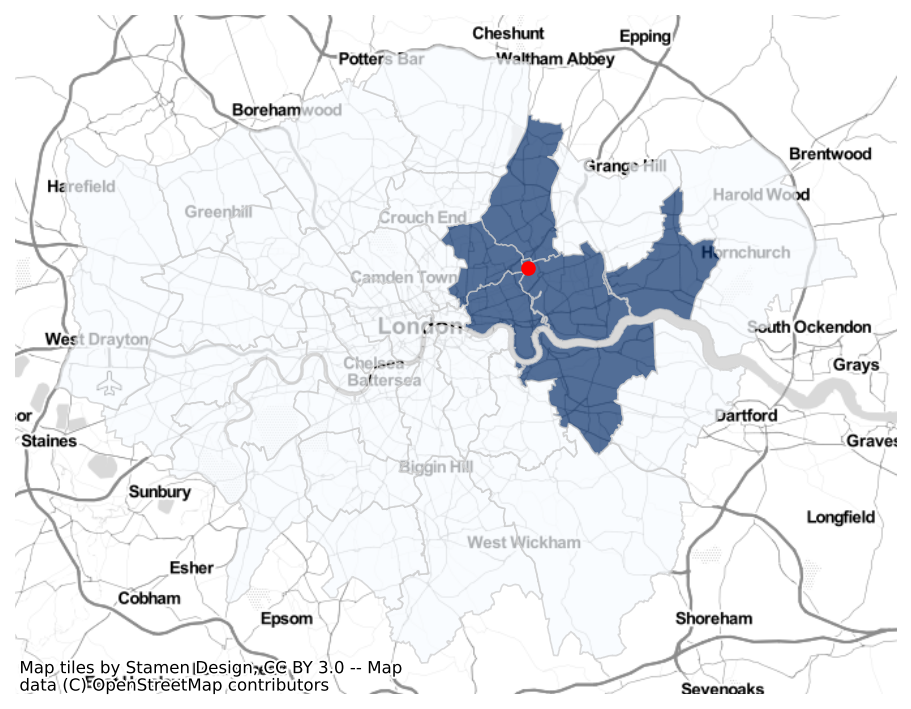
\includegraphics[scale=0.5]{east_london.png}
    \caption{\textbf{Map of East London in context.} Olympic venue labeled with red marker.}
    \label{fig:east_london}
\end{figure}

To accomplish this, London placed the Olympic Park in the the region of Newham, approximately in the center of East London (containing boroughs Barking and Dagenham, Greenwich, Hackney, Newham, Tower Hamlets, and Waltham Forest). Focusing on this aspect of the plan, we decided to compare this vision of "convergence" in East London with actual income and traffic statistics.

\subsubsection{Data Exploration}
Initially, we wanted to gain intuition on if the Olympics had had any widespread measurable effect at all on London. To do this, we first measured how proximity to the Olympic Park affected traffic, earnings, and economic activity.
%other stuff before this, as it may be odd to open with wasserstein like choropleth and distance or transportation. ADD MORE HERE? Especially traffic?

This measurement was conducted by finding the correlation coefficients between borough distance from the Olympic Park and a variety of other metrics, including London Underground use, number of economically active population, and income data.

All metrics yielded no or very weak correlation, with the maximum absolute correlation coefficient being 0.306. This suggests that the Olympics did not have a significant distance-mediated effect on London, contrary to what the Olympic planners might have hoped. However, this does not rule out the possibility of extremely local effects, which is further explored later.
\bigskip

We continued to explore if 2012 was vastly different from neighboring years, to confirm directly if the Olympics had a significant measurable effect on London. Using Wasserstein Distance metric, we calculated a pairwise heatmap to visualize how the distribution of hourly earnings changed between years.

\begin{figure}[H]
    \centering
        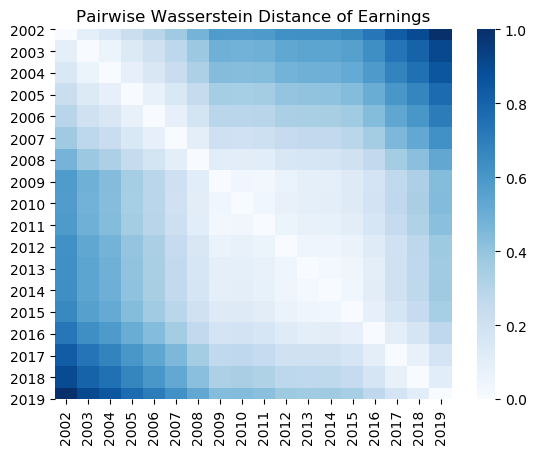
\includegraphics[scale=0.7]{justincome.png}
    \caption{\textbf{Pairwise Wasserstein Distance between every year from 2002-2019, using earnings data per borough for comparison}}
    \label{fig:earning_heatmap}
\end{figure}

Judging from these graphs, we suspected that the \textbf{Olympics did not create as dramatic an effect as originally hoped in the plan}, although the possibility of local effects remained. We continue by exploring several metrics separately.

\subsubsection{Further Analysis}

\begin{enumerate}
    \item \textbf{Economic activity does not change significantly in the years surrounding 2012}
    
    To obtain a higher dimensional understanding for each year with Topological Data Analysis, we combined the economic activity data and earnings by borough, along with physical distance in kilometers to the Olympic Park. Then, treating each of boroughs in each year as a point, we calculated the dimension 0 homology and then used Wasserstein Distance again to create the pairwise heatmap as seen below.
    
    \begin{figure}[H]
        \centering
            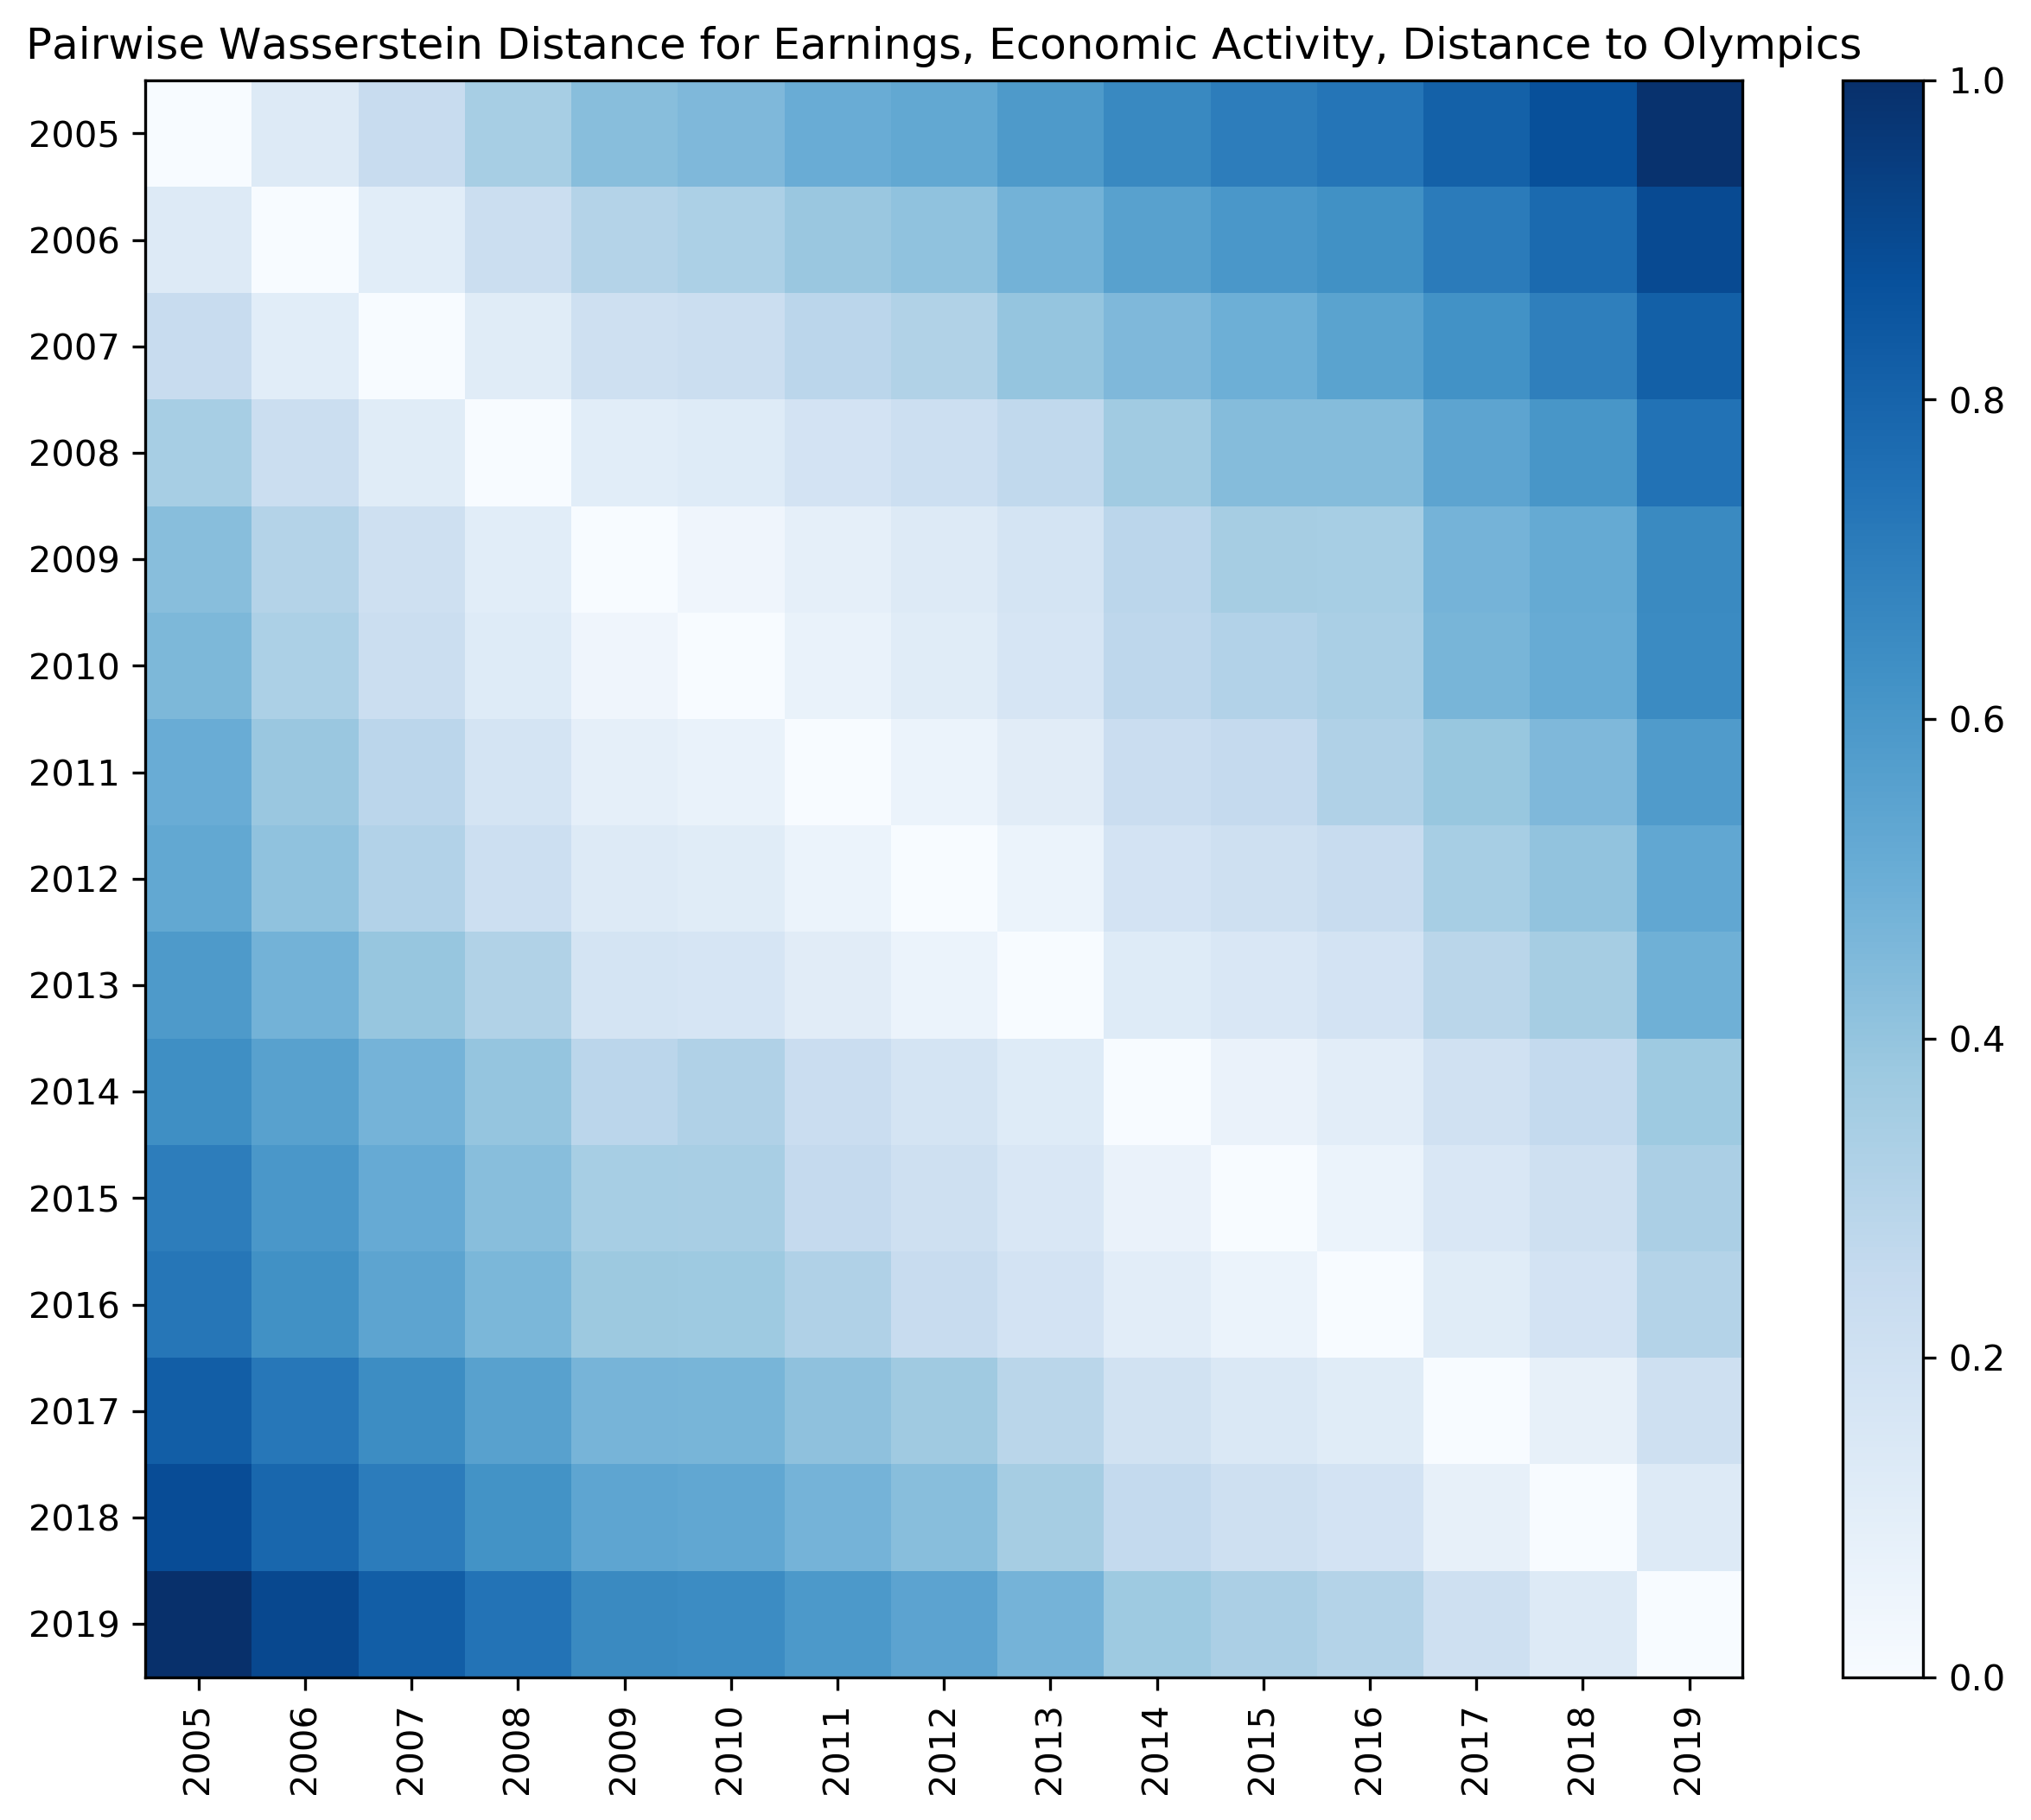
\includegraphics[scale=0.4]{econactincomedist.png}
        \caption{\textbf{Pairwise Wasserstein Distance between every year from 2002-2019}, using high dimensional points to represent boroughs with economic activity data, earnings, and distance to the Olympic Stadium}
        \label{fig:hybrid_heatmap}
    \end{figure}
    
    
    The equation for Wasserstein Distance is as follows: \[W_{q, p}(X, Y)=\inf _{s: X \rightarrow Y}\left(\sum_{x \in X}\|x-s(x)\|_{p}^{q}\right)^{\frac{1}{q}}\]
    
    which can also be intuitively described as the amount of work required to change one distribution into the other.
    
    Notice that between consecutive years the Wasserstein Distance is close to 0, showing that the shape did not change rapidly even around 2012. Therefore the shape and distribution economic status is not varying, so clearly the Olympics cannot be producing massive fluctuation. 
    
    This agrees with the earlier heatmap in Figure \ref{fig:earning_heatmap}, showing that even when including factors besides earnings, we still did not see pronounced contrast in the overall shape and distribution of economic markers in the years near 2012.
    
    \item \textbf{Income growth increases in the immediate locality of the Olympics, but the income gap does not close}
    
    Another one of the goals of the 2012 London Olympics was the narrowing of the income gap between East London and the remainder of London. Initially, this goal seems to have some merit based on an initial study of the chloropleth in Figure \ref{fig:income_chloropleth}.
    
    \begin{figure}[H]
        \centering
            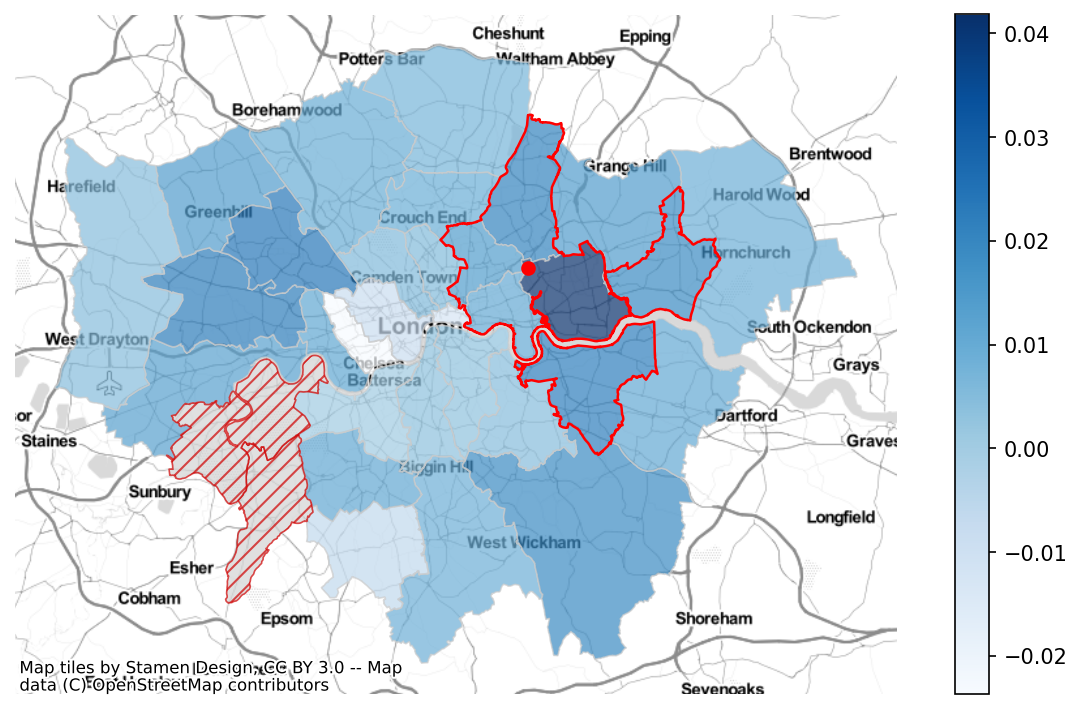
\includegraphics[scale=0.5]{income_slope.png}
        \caption{\textbf{Choropleth of normalized change in income growth rate before and after the 2012 Olympics per region.} Olympics venue location highlighted with a red dot, with East London outlined in red. Missing data denoted by red hatches on grey.}
        \label{fig:income_chloropleth}
    \end{figure}
    
    Figure \ref{fig:income_chloropleth} shows the normalized change in income growth rate, as measured using linear regression, between pre and post-Olympics years. The coefficient of linear regression was chosen to measure growth rates due to its resistance to year-over-year outliers and greater explanatory power for a range of years. In this case, positive values mean that the average year-over-year growth rate in income increases following the 2012 Olympics, with negative values implying decrease.
    
    In Figure \ref{fig:income_chloropleth}, we find that the borough of Newham (located immediately underneath the red dot) has the highest change in income growth rate following the Olympics, which initially lends hope to London's goal of narrowing the East London income gap. However, on a larger scale as seen in Figure \ref{fig:median_income}, the data tells a different story.
    
    \begin{figure}[H]
        \centering
            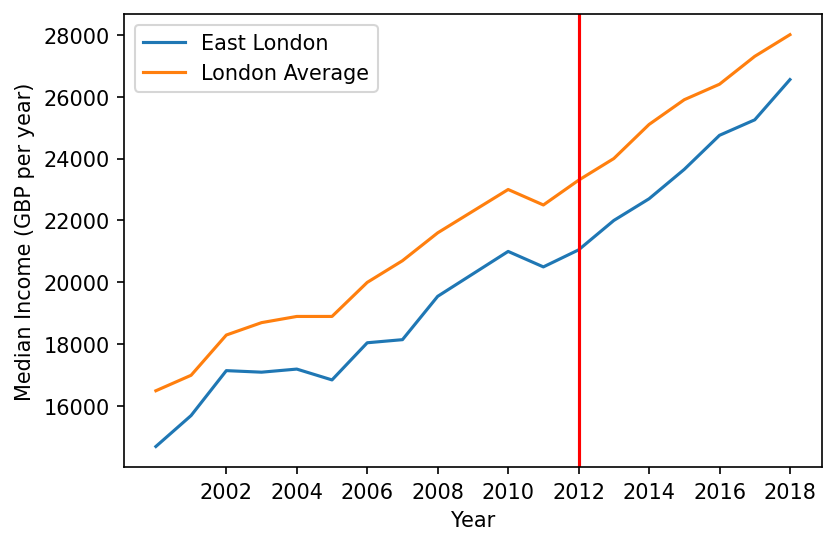
\includegraphics[scale=0.5]{median_income.png}
        \caption{\textbf{Median income for both East London and London in its entirety over time.} Data ranges between year 2000 and 2018, with a red vertical line indicating the occurrence of the Olympics during 2012.}
        \label{fig:median_income}
    \end{figure}
    
    Figure \ref{fig:median_income} compares median income between East London and the London Average. We find that the median income gap barely changes 2012 onwards, which suggests that, despite local effects, the Olympics in London did not have larger scale economic effects.
    
    One may argue that the Olympics may have had an effect as soon as London's hosting of the Olympics was originally confirmed, before the Olympics occurred. However, this happened in 2005, yet relatively little change occurs between 2005-2012 as well.
    
    In summary, \textbf{the Olympics did result in limited local effects, while general income gap momentum remained exactly the same.}
    
    \item \textbf{Traffic growth rate in East London is only temporarily accelerated by the Olympics}
    
    To further investigate London's attempts to reinvigorate East London with the Olympics, we analyzed traffic moving through each borough. Specifically, we used annual entry and exit statistics for London Underground stations as a proxy for total traffic.
    
    We began by generating a choropleth of normalized change in London Underground traffic between pre and post-Olympic data using linear regression in a similar method as in the above section.
    
    \begin{figure}[H]
        \centering
            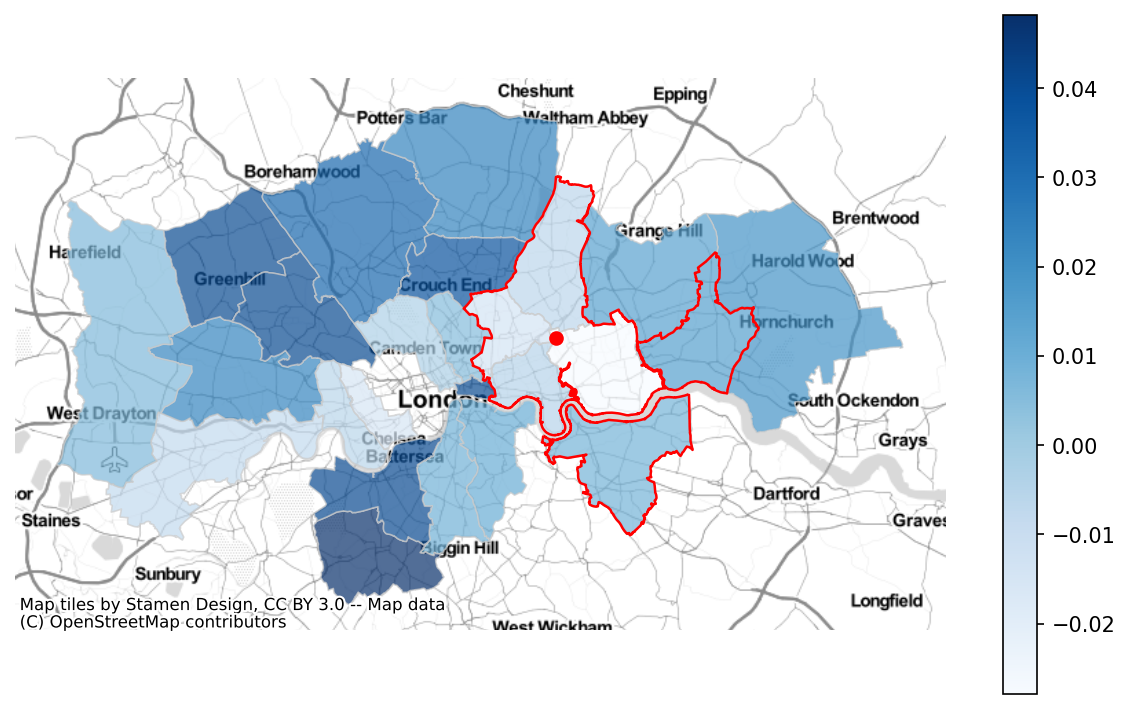
\includegraphics[scale=0.45]{underground_slope.png}
        \caption{\textbf{Choropleth of normalized change in London Underground traffic before and after the 2012 Olympics per region.} Olympics venue marked with red dot, with East London outlined in red. Some boroughs missing due to lack of Underground stations.}
        \label{fig:underground_slope}
    \end{figure}
    
    This choropleth, as seen in Figure \ref{fig:underground_slope}, clearly shows predominantly negative changes in growth rate in East London following the London Olympics, at a stark contrast to the majority of the city, with far more positive changes in growth rate.
    
    \begin{figure}[H]
        \centering
            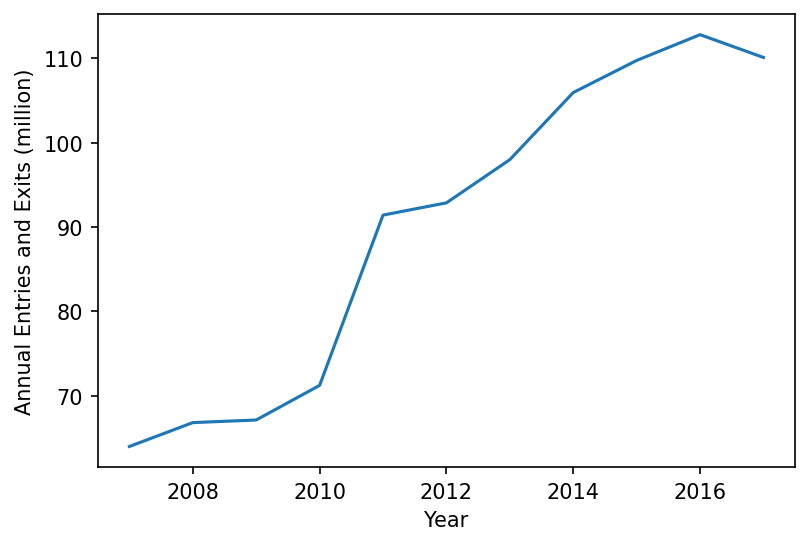
\includegraphics[scale=0.5]{newham_activity.png}
        \caption{\textbf{Newham annual London Underground annual entries and exits over time.} Data ranges from 2007 to 2017, with the Olympics occurring in 2012.}
        \label{fig:newham_activity}
    \end{figure}
    
    Furthermore, this trend is even more visible in a more detailed analysis of Newham's underground data over time in Figure \ref{fig:newham_activity}. In fact, London Underground ridership shows extremely slow to no growth following 2014, visually corroborating the quantifiable decline in Figure \ref{fig:underground_slope}.
    
    This negative change in growth rate can be interpreted as a very quick return to pre-Olympic traffic growth rates in East London after a temporarily artificially inflated period during Olympic development. In fact, the Olympics in this case can be seen as only \textbf{temporarily accelerating the existing trend of slow growth}.
    
    This suggests that \textbf{the surge of traffic from the Olympics is short-lived and artificially created}, inherently leading to \textbf{no change in long-term outlook}.
\end{enumerate}
    
\subsubsection{Summary}
The plan for the Olympics did not quite attain its objectives, with milder growth than anticipated overall and the separation between East London and its counterparts remaining essentially the same. However, boroughs in East London did improve economically, which lends support to the argument that the Olympics affect neighboring locations. However, this improvement is insignificant in the context of long term trends. With these findings, we concluded that the Olympics did not disrupt general trends in income and economic activity, and that the Olympics were slightly beneficial but would not have a strong influence long term.

\subsection{Vancouver 2010}

The 2010 Winter Olympic games were thought by many Canadians to be a jump start to firmly launch Vancouver onto the global stage. Broadcasting the economic goal set for the Vancouver Games, Stephen Harper, the PM of Canada, had said: 
\begin{displayquote}
“Mark my words, someday historians will look back at Canada's growing strength in the 21st century and they will say that it all began right here, on the West Coast, with the best Winter Olympic Games the world has ever seen"\cite{olympics}
\end{displayquote}
 Were these goals for the Vancouver games actually met? A closer look at economic data may suggest that the Olympics may have missed their high-water mark. 

\subsubsection{Data Exploration}

    We begin our analysis of the Vancouver games by looking at construction company formation, a strong metric of growth and investment in a given region. In fact, by Olympic budget, 81.6\% of costs are devoted to construction. In the below graphics, in the years leading up to the winter Olympics (2009-2010), there was substantial year over year increase in the creation of new construction businesses. The largest increases (blue) were discovered in areas closest to the Olympic venues, namely Whistler and Vancouver.
    
    \begin{figure}[H]
        \centering
            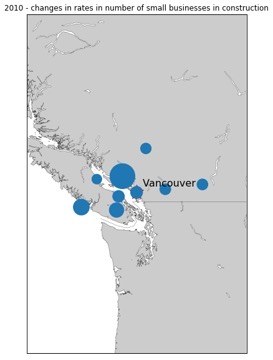
\includegraphics[scale=0.45]{Vancouver_map_2010.JPG}
            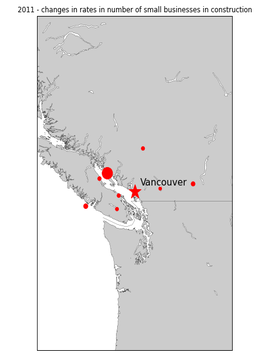
\includegraphics[scale=0.46]{vancouver_map_2011.png}
        \caption{\textbf{Vancouver map of rate of change in number of small businesses in construction - 2010 and 2011 YoY change.} Blue represents Positive YoY Change, Red represents negative YoY change. Area of circles represents magnitude in change}
        \label{fig:Vancouver_map}
    \end{figure}
    
    We continued to look at region popularity metrics, which would be indicative of Vancouver's planned jump to the global stage. To do this, we used lodging revenues as a rough estimate of both tourist volume and spending in these areas. During the initial data analysis, the British Columbia lodging rental revenue data had a large number of missing entries in the years from 2010-2019, which limited its use in our analysis. In order to deal with this, we removed any cities which had incomplete data and would corrupt substantial cities. Continuing with the analysis, we aggregated revenue data across lodging type and crafted individual time series for the each of the regions. Once the data had been aggregated and the regions with corrupted data had been removed, we then decided it would be best to limit which towns we retain in our analysis and decided that proximity to the Olympic venues in Whistler and Vancouver would be the best metric. Using a 4-hour drive as a distance cut off we were then able to construct a Lodging Revenue analysis of the Vancouver area.
    
    We noticed that the main venue areas of Whistler as well as Vancouver saw dramatic spikes in lodging revenue during the months of the Winter Olympics However, as equally impressive as the spike in lodging revenue is the decrease in lodging revenue in the subsequent months.(Figure \ref{fig:Vancouver_Room_rev}). Therefore we suspect that \textbf{initial geographic benefits of hosting an Olympics are noticeable, however any substantial long term effect diminishes}
    
    \begin{figure}[H]
        \centering
            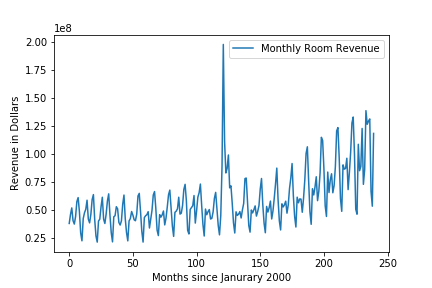
\includegraphics[scale=0.55]{Vancouver_Area_Room_Revenue.png}
        \caption{\textbf{Vancouver Area Monthly Room Revenue}}
        \label{fig:Vancouver_Room_rev}
    \end{figure}
    
    \begin{figure}[H]
        \centering
            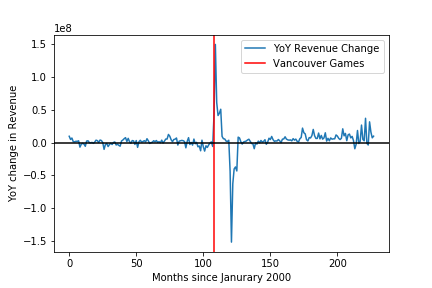
\includegraphics[scale=0.55]{Vancouver_Area_Deseasoned_Room_Revenue.png}
        \caption{\textbf{Vancouver Area Monthly Room Revenue - YoY Change}}
        \label{fig:Vancouver_Room_rev_YoY}
    \end{figure}
    
    For a clear, non-seasonal, picture of the year over year changes in lodging related revenue, look at following graph which plots the year over year change in lodging revenue (Figure \ref{fig:Vancouver_Room_rev_YoY}).The lackluster growth is plain, revealing the lack of year over year growth in rental related revenue. For the next 5-6 years, the lodging revenue of the Vancouver/Whistler areas as well as the greater Vancouver area returned to pre-Olympics levels and by proxy highlights that tourism and spending in those areas did not increase either. This mediocre economic performance is further emphasized by the construction business decline (red) established in the years following the Olympics namely 2011-2012(Figure \ref{fig:Vancouver_map}, right side), emphasizing how the Olympics stimulus did not permeate throughout the ensuing years. 
    
\subsubsection{Further Analysis}  
\begin{enumerate}
    \item \textbf{Any visibility gained by the Olympic games did not spur any substantial growth in travel to the Vancouver }
    
    Another metric to judge how the areas closest to Vancouver had been affected both during and after the Olympics would be the visits to the region. To precisely define Vancouver Region, we analyzed towns within a 4 hour drive of either Vancouver or Whistler(the Olympic venues). As shown in Figure \ref{fig:Vancouver_Monthly_YoY}, we can see that the de-seasoned plot of the year over year visits points to similar growth rates to before the 2010 Vancouver games, pointing to no material gains from hosting the Winter Olympics. 
    
    \begin{figure}[H]
        \centering
            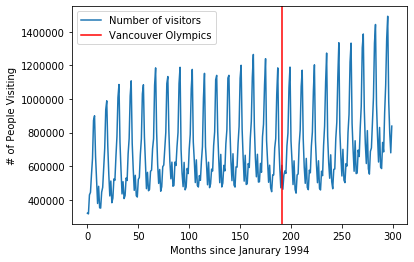
\includegraphics[scale=0.6]{Vancouver_Monthly_Visitors.png}
        \caption{\textbf{Vancouver Monthly Visits}}
        \label{fig:Vancouver_Monthly}
    \end{figure}
    
    \begin{figure}[H]
        \centering
            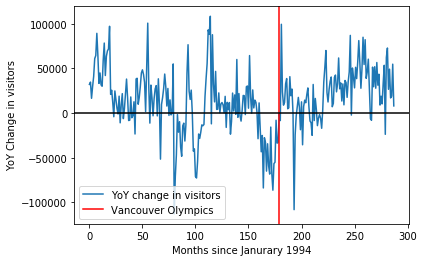
\includegraphics[scale=0.6]{Vancouver_Monthly_Visitors_YoY.png}
        \caption{\textbf{Vancouver Monthly Visits - YoY change}}
        \label{fig:Vancouver_Monthly_YoY}
    \end{figure}
    
   \subsubsection{Summary} 
    
    With the lack of increased growth in visits to the region, one could argue that the goal of ‘putting Vancouver on the map' failed, as the Olympics did not significantly increase the popularity of the region as a destination. Couple this with the relatively lackluster economic performance seen in both the tourism and construction industries following the Olympic games, and the benefits of these Olympic games diminishes even further. Taken together, these analyses highlight how the 2010 Olympics failed propel Vancouver forward and ultimately fell short of the lofty ideal proposed by the Prime Minister and the broader Canadian public. 

\end{enumerate}

\subsection{Rio 2016}

Similar to many of the previous Olympic games, Rio had high hopes of increasing visibility and travel to the region. Rio’s organizing committee had the objective to increase visitors to Brazil both during the games and throughout the end of September 2016. The committee set this number as high as 82\%, resulting in a potential increase of 350,000-500,000 additional visitors. Furthermore, the president of Brazil's tourism board went as far as to suggest that leveraging the increased visibility of Brazil could yield more tourists in the long term.\cite{theconversation} For perspective on the full situation, according to an article published by the AP, this gamble was said to cost a total of \$13 billion USD, \$10 billion more than what was estimated by the Olympic organizing committee.\cite{ap} This gamble to increase tourism is quite perplexing if you take into account the climate of Brazil's tourism industry at the time. In the below graph, we see that the tourism industries in both Rio and Brazil as a whole had been growing steadily since 2006 up until January 2016 (Figure \ref{fig:Brazil_Rio_Tourism}). When the existing growth is taken into account, it seems like the goal of using the Olympics for tourism industry stimulus is unnecessary and potentially already a waste. Regardless of the wisdom in making that choice, was Brazil able to realize the additional growth it sought in its tourism industry?

\subsubsection{Data Exploration}

    Unpacking the goals laid out by the Rio Olympic Committee, we will first verify if the games were able to increase international visits to Brazil. Looking at the graph below, we are able to view the year over year change in International visits, where the red vertical line is the Rio Olympic games. The month of the Olympic games, Brazil did see a year over year increase of ~200,000 visitors, however, their goal was an increase of 350,000-500,000 visits. What is even more striking is that immediately following the Olympic games, international visits fell off sharply (~200k) and virtually erased any momentum gained from the games in the previous two months. In the next two years following the Olympic games, international visits stayed relatively close to their previous levels oscillating across the 0\% y/y growth line. This analysis helps shape the conclusion that Brazil in fact did not meet the Olympic committees’ goals, as we observe that \textbf{international visits to Brazil during and following the Olympics fell short of expectations}
    
    \begin{figure}[H]
        \centering
            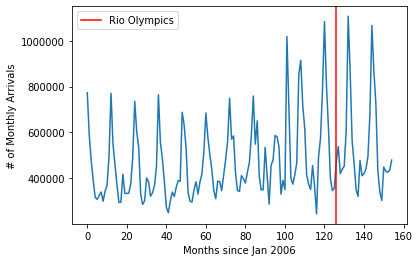
\includegraphics[scale=0.6]{Brazil_Arrivals.png}
        \caption{\textbf{Brazil International Arrivals - Monthly}}
        \label{fig:Brazil_Arrivals}
    \end{figure}
        
    \begin{figure}[H]
        \centering
            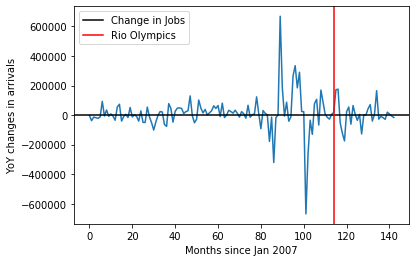
\includegraphics[scale=0.6]{Brazil_Arrivals_deseasoned.png}
        \caption{\textbf{Brazil International Arrivals - YoY Change}}
        \label{fig:Brazil_Arrivals_deseasoned}
    \end{figure}    
    
    We now switch to a comparison of the economic impact of the games on both Rio and Brazil as a whole. The below chart plots the monthly tourism related jobs in both Brazil as well as just Rio. Along with this chart we plotted two vertical lines which we believe indicate points of interest, the Zika virus epidemic (black line) and the Brazil 2016 games (red line). It is clear in the below graph that both Brazil and Rio share similar trajectories in Tourism industry growth, however what is intriguing is the discrepancy following the Zika virus outbreak. 
    
    \begin{figure}[H]
        \centering
            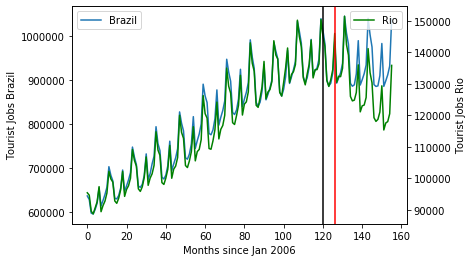
\includegraphics[scale=0.55]{Brazil_and_Rio_Tourism_Jobs.png}
        \caption{\textbf{Brazil and Rio Tourism Jobs by month since 2006}}
        \label{fig:Brazil_Rio_Tourism}
    \end{figure}

    \subsubsection{Further Analysis}
\begin{enumerate}
     \item \textbf{The Olympics accelerated the decline of the tourist industry in Rio relative to the rest of Brazil}
     
     
    Visually it appears that the tourism industry in Rio is worse than Brazil as a whole, however to show that the decline in tourism employment in Rio was statistically worse than the decline seen in all of Brazil, we fit a Moving Average model to the time series, which would provide us with tools to conduct inference on the two trends. In order to standardize the scale of the data we first converted each time series into a percentage change from the January 2016 peak (shown by the black horizontal line); this peak also happened to coincide with the popularization of the Zika virus in the country. Then we modeled the \% change in tourism employment, both in Brazil and Rio, from the peak of the market in January. Additionally, both series have been differenced in order to remove any linear trends in the data, with the purpose of making the time series stationary. 
    
    Having standardized and de-trended the data we then used an augmented Dick-Fuller test to confirm stationarity of our differenced time series. Given the covariance stationarity of the series, it is often appropriate to use either an  MA or AR models.As will be discussed later it will be beneficial for us to model this as an Moving-Average model. We then fit a seasonal MA(7) model to the series, which we selected based on the AIC score of the model versus comparable models.  The seasonality was selected to be 12, both matching intuitive reasoning as well as a spectral decomposition on the data (Figure \ref{fig:Spectral_Plot}, noting leakage in the spectral estimate).
  
   \begin{figure}[H]
        \centering
            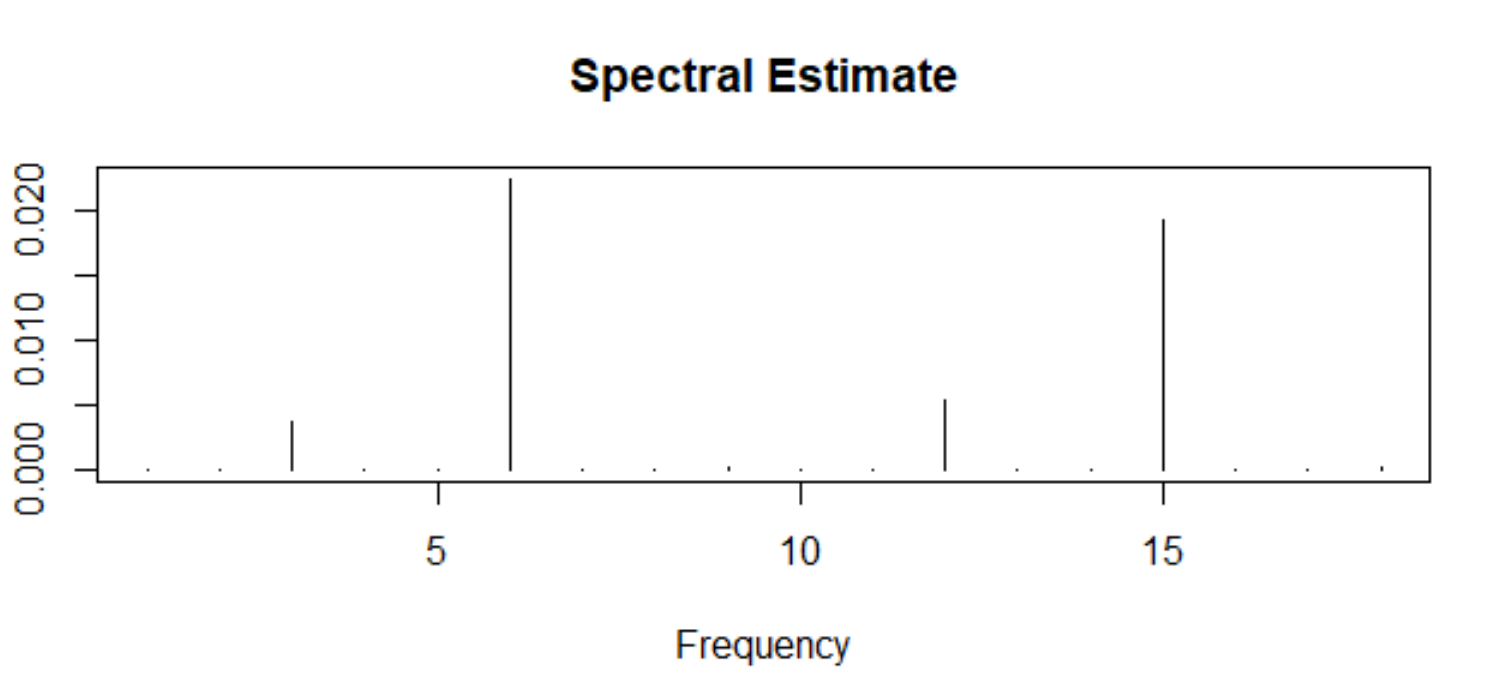
\includegraphics[scale=0.5]{Spectral_estimate.PNG}
        \caption{\textbf{Periodogram of the differenced Brazil and Rio Employment Data}}
        \label{fig:Spectral_Plot}
    \end{figure}  
    
    
  By constructing the time series as a seasonal MA model, we can interpret the intercept of both models as the slope of the linear trend from the previously undifferenced time series. Finally, assuming normality of the error process we conducted a difference in means hypothesis test comparing the mean \% decline in the Brazil tourism employment data against the Rio tourism employment data. The specifics of the test are as follows:
    \begin{align*}
        H_o&: \mu_1 \geq \mu_2\\
        H_a&: \mu_1 < \mu_2
    \end{align*}
    where $\mu_1$ is the mean \% employment change from the peak for the Rio data and $\mu_2$ is the mean \% employment change from the peak for the total Brazil data.  We can now form our test statistic as,
    \[T = \frac{\hat{\mu}_{1} - \hat{\mu}_{2}}{\sqrt{\frac{\hat{\sigma}_{1}^{2}}{n_1}+\frac{\hat{\sigma}_{2}^{2}}{n_2}}}\]
    We can now reject our null hypothesis if,
    \[T < -z_{\alpha}\]
    Upon fitting the optimal MA model, constructing this test statistic using the intercepts and setting $\alpha = .05$, we were able to reject the null hypothesis and can conclude that $\mu_1 < \mu_2$. We can comfortably conclude that following the January 2016 peak in tourism employment, the tourism industry in Rio under performed the greater tourism industry in Brazil.
    
\end{enumerate}

    
\subsubsection{Summary}
    
    Although it is graphically obvious that the decline in tourism employment started before the Rio games, what is still interesting is the relative performance of Rio vs Brazil as a whole. Given that the previous hypothesis test showed that the linear trend following the 2016 peak in tourism employment was worse in Rio vs all of Brazil, we speculate that Rio may have over invested in their tourism industry, expecting an increase of visitors due to the Olympics. Regardless of the cause of underperformance, the Rio Olympics clearly did not help the region sustain any growth in their tourism industry. Although Brazil as a whole had a decrease in visits and tourist activity following Zika virus concerns, the underperformance of Rio in particular suggests that the Olympics could not prevent the downward slump and draws doubt as to whether or not the \$13 billion dollar investment may have been worth it.


\section{Conclusion}
%also maybe acknowledge how vancouver is winter so it may be different + other details

In the wake of the three Olympics, we have observed every time that the projected windfall did not occur. In London, it there were moderate returns, but not quite to the level anticipated. In Vancouver, there were brief spikes, but no tangible gain afterwards. Finally in Rio, with the Zika outbreak, and recent recession, the Olympics could not prop up the economy and may have even decreased tourism employment in Rio. Looking at common themes between scenarios, we observed that proximity to the Olympics did result in increased activity, but not sustained, and not as substantially as desired. Additionally, the economic trends from before the Olympics consistently outweighed the effects of the Olympics and persisted throughout the years following. Therefore, we advise that it is safer to treat the Olympics as a temporary and geographically limited benefit, and not to over-invest by expecting expansive economic growth.



% Here's where you specify the bibliography style file.
% The full file name for the bibliography style file 
% used for an ASME paper is asmems4.bst.
\bibliographystyle{asmems4}

\begin{thebibliography}{12}

\bibitem{ap}Brito, R. (2017, June 14). AP Analysis: Rio de Janeiro Olympics cost \$13.1 billion. Retrieved July 19, 2020, from \url{https://apnews.com/d1662ddb3bae4d2984c\\a4ab65012be78/AP-Analysis:-Rio-de-Janeiro-Olympics-cost-\$13.1-billion#:~:text=RIO DE JANEIRO (AP) —,of public and private money}

\bibitem{theconversation}Duignan, M. B. (2020, February 18). Why Rio 2016 may not bring the tourism boost Brazil hopes. Retrieved July 19, 2020, from \url{https://theconversation.com/why-rio-2016-may-not-bring-the-tourism-boost-brazil-hopes-64145}

\bibitem{bloomberg}O'Sullivan, F. (2017, November 20). The London Olympics Didn't Improve Life in East London. Retrieved July 19, 2020, from \url{https://www.bloomberg.com/news/articles/2017-11-20/the-london-olympics-didn-t-improve-life-in-east-london}

\bibitem{london_asm}Relighting the torch: Securing the Olympic legacy. (2017, November). Retrieved from \url{https://www.london.gov.uk/sites/default/files/\\convergence\_short\_report\_final.pdf}

\bibitem{olympics}Staging the Olympic Winter Games Knowledge Report. (2010, September). Retrieved July 19, 2020, from \url{https://stillmed.olympic.org/Documents/Reports/\\Official Past Games Reports/Winter/EN/Staging-the-Games.pdf}

\end{thebibliography}


\appendix                                    
\section{Other Analysis Attempts}

We wanted to see how proximity to Olympic venues affected growth in the economy. To do that, we constructed a correlation heatmap on the year on year rate change in the number of small businesses in the different industries in British Columbia before and after the Olympics. While this it is striking to see that the YoY number of businesses is highly correlated among all the different industries in the year 2009-2010 leading to the Olympics, 2010-2011 showed that some industries plummeted post Olympics. (Figure \ref{fig:Correlation_circle})

\begin{figure}[H]
    \centering
        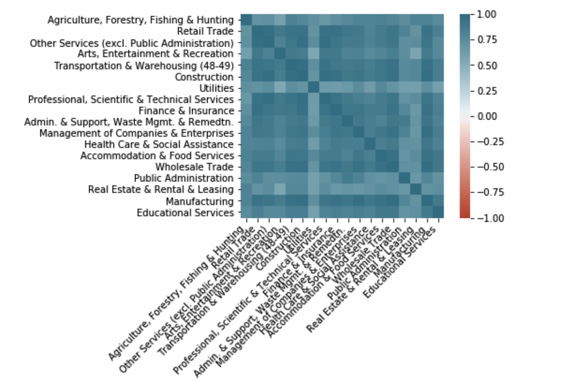
\includegraphics[scale=0.3]{Correl_2010.jpg}
        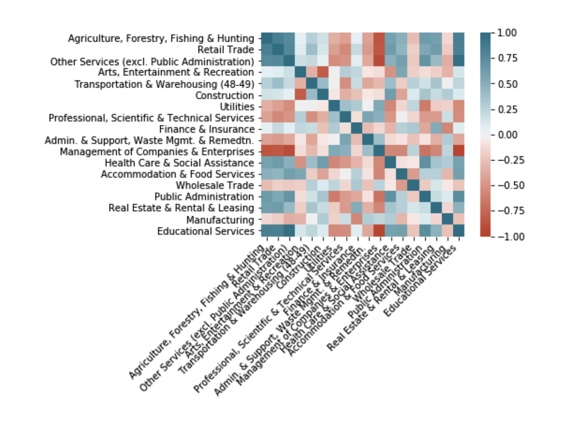
\includegraphics[scale=0.3]{Correl_2011.jpg}
    \caption{\textbf{Correlation of the YoY number of small businesses in the different industries in British Columbia}}
    \label{fig:Correlation_circle}
\end{figure}   

To further understand how each industries are correlated, we drew a unit circle, with each arrows being the project of the YoY number of small businesses in the different industries in British Columbia on the first 2 principal components in 2011. Positively correlated variables are grouped together while negatively correlated variables are positioned on opposite sides of the plot origin. As arrows representing 'Construction' and 'Transportation' are pointing in the same direction, they belong to the group of industries that saw a decline right after the Olympics in British Columbia. 

\begin{figure}[H]
    \centering
        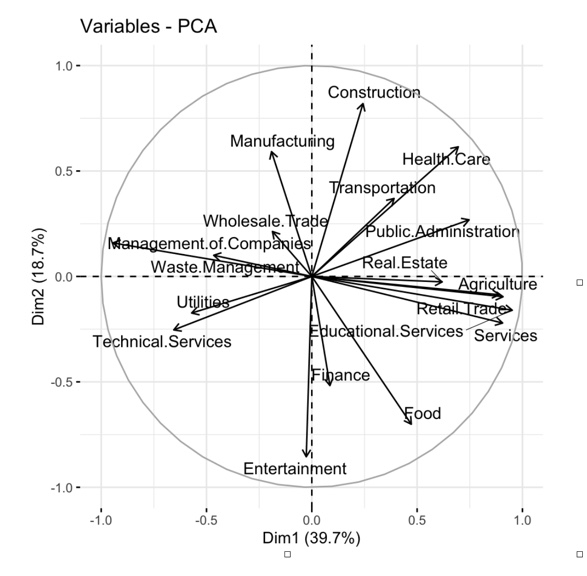
\includegraphics[scale=0.33]{Correlation circle.jpg}
    \caption{\textbf{Projection of the YoY number of small businesses in the different industries in British Columbia on the first 2 principal components - 2011}}
    \label{fig:Correlation_circle}
\end{figure}

\end{document}

